\documentclass{beamer}
\usepackage[utf8]{inputenc}

\usepackage{utopia} %font utopia imported

\usetheme{Madrid}
\usecolortheme{default}

\definecolor{RedCIMAT}{rgb}{0.44921875, 0.13671875, 0.234375} % UBC Blue (primary)
\usecolortheme[named=RedCIMAT]{structure}

%------------------------------------------------------------
%This block of code defines the information to appear in the
%Title page
\title[Avance de Tesis] %optional
{Métodos de Análisis de Secuencias basados en Aprendizaje Profundo en problemas de Visión y Procesamiento de Imágenes}

\subtitle{Estimación de Pose y Clasificación de Imágenes}

\author[Esaú Peralta] % (optional)
{Óscar Esaú Peralta Rosales\inst{1} \and Dr. Mariano Rivera Meraz\inst{1}}

\institute[CIMAT] % (optional)
{
  \inst{1}%
  Centro de Investigación en Matemáticas A.C.
}

\date[Julio 2021] % (optional)
{Avance de Tesis}

\logo{
\includegraphics[height=0.7cm]{logo.jpg}}
%End of title page configuration block
%------------------------------------------------------------



%------------------------------------------------------------
%The next block of commands puts the table of contents at the
%beginning of each section and highlights the current section:

\AtBeginSection[]
{
  \begin{frame}
    \frametitle{Table of Contents}
    \tableofcontents[currentsection]
  \end{frame}
}
%------------------------------------------------------------


\begin{document}

%The next statement creates the title page.
\frame{\titlepage}


%---------------------------------------------------------
%This block of code is for the table of contents after
%the title page
\begin{frame}
\frametitle{Tabla de Contenido}
\tableofcontents
\end{frame}
%---------------------------------------------------------


\section{Motivación de la Tesis}


%---------------------------------------------------------
%Changing visibility of the text
\begin{frame}
\frametitle{Motivación de la Tesis}
Con el auge de los Transformes como modelos de procesamiento de información secuencial, el trabajo
de esta tesis ha sido dirigido en explorar dichos modelos en áreas fuera del Procesamiento del
Lenguaje Natural.\\~\

Finalmente se propone una variante enfocado en aumentar la capacidad receptiva de las cabezas de
atención permitiendo mayor flexibilidad al no estar ligada al tamaño de embedding predefinidos.\\~\

Las experimentaciones del funcionamiento del modelo se realizan en los siguientes problemas:
\begin{itemize}
    \item Predicción de Pose 2D en humanos sobre imágenes
    \item Predicción de Pose 3D en humanos (Monocular, Desacoplado)
    \item ViT y Clasificación de Enfermedades Comunes de Tórax (INAOEP, CIMAT, IMSS)
\end{itemize}
\end{frame}

%---------------------------------------------------------

\section{Descripción de los Problemas}

%---------------------------------------------------------
%Highlighting text
\begin{frame}
\frametitle{Estimación de Pose 2D y 3D en Humanos}

\begin{itemize}
    \item 2D: Dada una imágen estimar las posiciones de las articulaciones de la persona en cuestión
          sobre la imagen.
    \item 3D: Dada una imagen estimar las posiciones de las articulaciones dentro de un marco de
          referencia que mejor ajuste la posición espacial de la persona en cuestión.
\end{itemize}

\begin{columns}
\column{0.5\textwidth}
\begin{figure}[htbp]
    \centerline{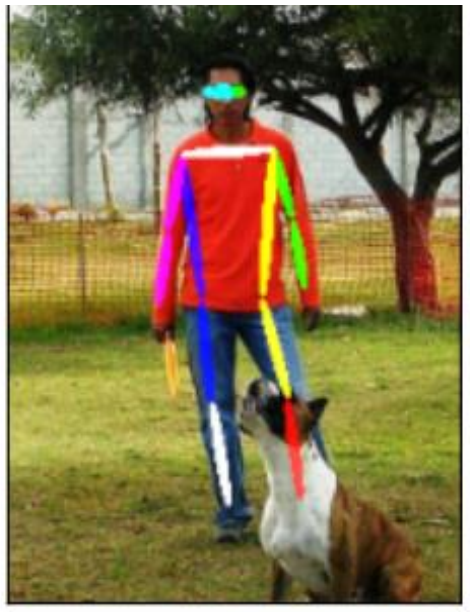
\includegraphics[height=1in]{images/example_2D.png}}
    \caption{Estimación de Pose 2D}
    \label{fig:ie2d}
\end{figure}

\column{0.6\textwidth}
\begin{figure}[htbp]
    \centerline{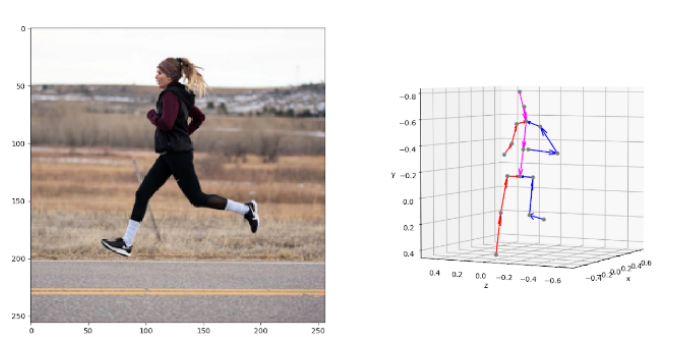
\includegraphics[height=1in]{images/example_3D.png}}
    \caption{Estimación de Pose 3D}
    \label{fig:ie3d}
\end{figure}
\end{columns}
\end{frame}
%---------------------------------------------------------


%---------------------------------------------------------
%Two columns
\begin{frame}
\frametitle{Estimación de Pose 2D y 3D en Humanos}

\begin{columns}

\column{0.4\textwidth}
Esqueleto
\begin{itemize}
    \item 17 articulaciones
    \item 16 huesos \\~\
\end{itemize}

Datasets
\begin{itemize}
    \item Human 3.6M
    \item COCO 2017
\end{itemize}

\column{0.6\textwidth}
\begin{figure}[htbp]
    \centerline{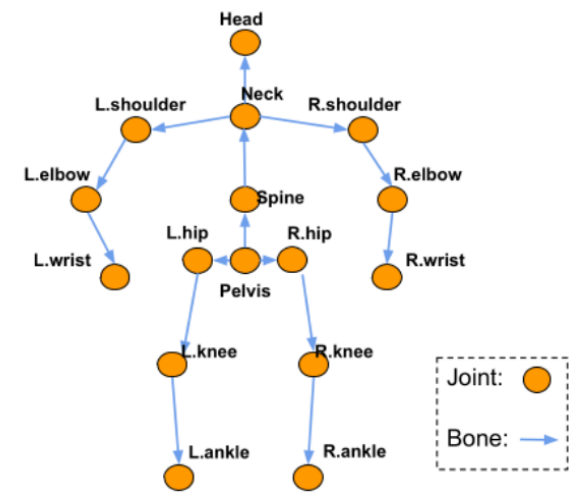
\includegraphics[height=1.5in]{images/joints.png}}
    \caption{Articulaciones usadas en tareas de Estimación de Pose en Humanos. Imagen tomada del
    artículo "Anatomy-Aware 3D Human Pose Estimación en Videos"}
    \label{fig:joints}
\end{figure}

\end{columns}

\end{frame}
%---------------------------------------------------------

%---------------------------------------------------------
%Two columns
\begin{frame}
\frametitle{Detección y Clasificación de Enfermedades Comunes de Tórax}

% La examinación por Rayos-X es uno de los métodos más comunes para la detección y diagnóstico de
% enfermedades que atacan la zona toráxica.

\begin{columns}
\column{0.5\textwidth}
\begin{itemize}
    \item Trabajo colaborativo entre CIMAT, INAOE e IMSS.
    \item Modelo clasificador para la detección de 15
          padecimientos incluyendo COVID-19.
    \item Se realiza la comparativa de un modelo basado en ViT con las modificaciones antes
          mencionadas.
\end{itemize}

\column{0.5\textwidth}
\begin{figure}[htbp]
    \centerline{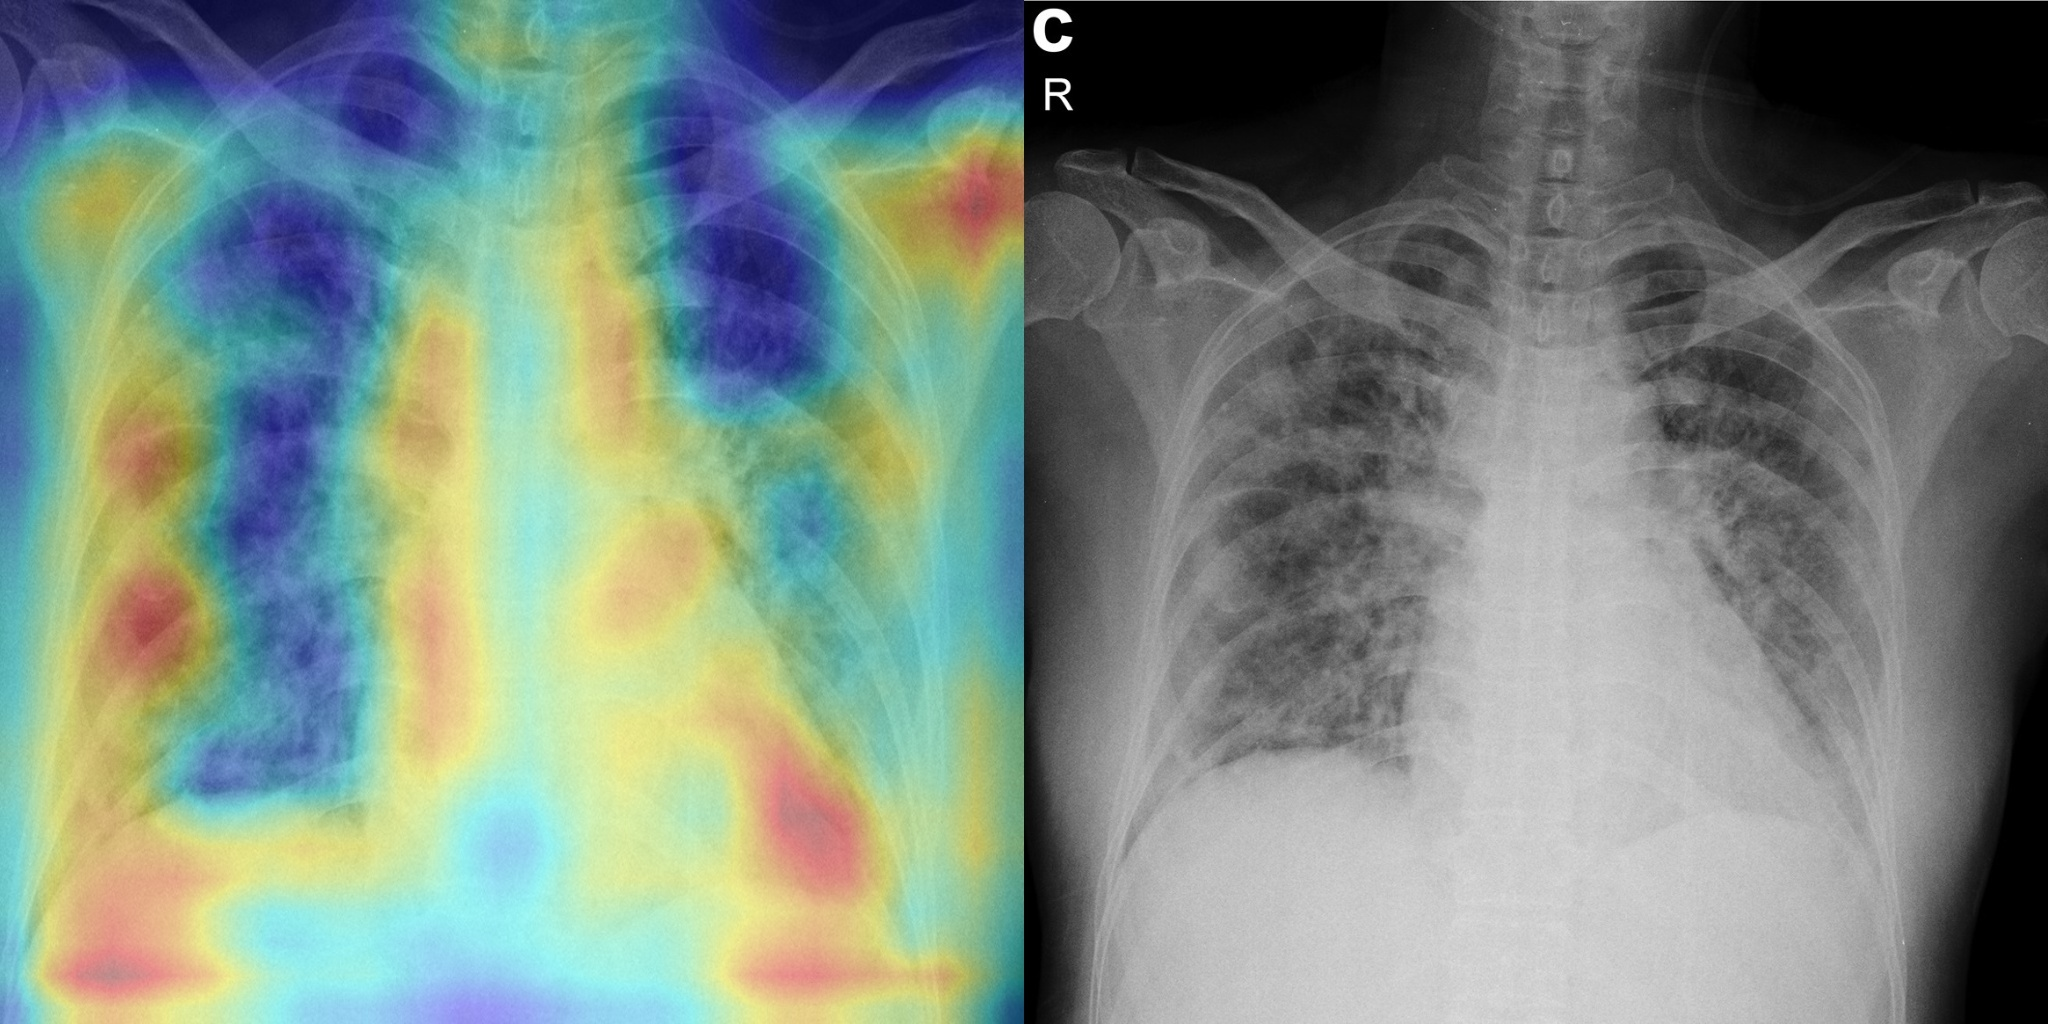
\includegraphics[width=1.5in]{images/lung_covid.jpg}}
    \caption{Áreas Afectadas por COVID-2019 detectadas por el modelo usando GradCam.}
    \label{fig:lung}
\end{figure}
\end{columns}

\end{frame}
%---------------------------------------------------------

\section{Modelos}

%---------------------------------------------------------
\begin{frame}
\frametitle{Modelo Estimación de Pose 2D}

\begin{figure}[htbp]
    \centerline{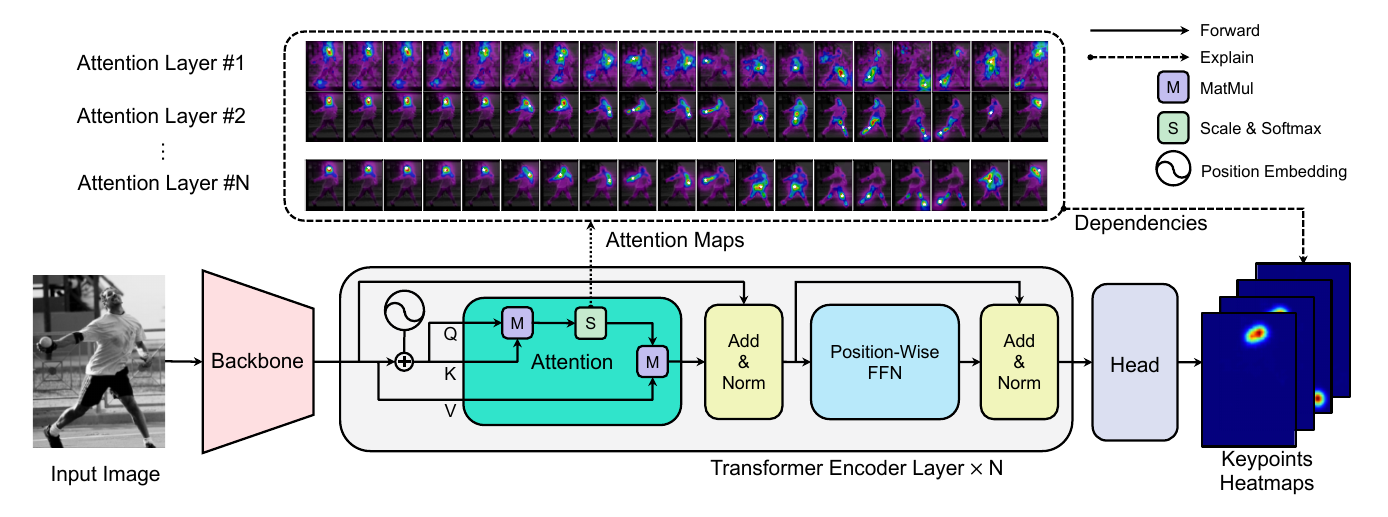
\includegraphics[width=5.0in]{images/model_2D.png}}
    \caption{Modelo Predicción de Pose 2D. Al igual que ViT usa capas con Decoders con entrada las
             características obtenidas por un modelo convolucional usado como Backbone}
    \label{fig:m2d}
\end{figure}

\end{frame}
%---------------------------------------------------------

%---------------------------------------------------------
\begin{frame}
\frametitle{Modelo Estimación de Pose 3D}

\begin{figure}[htbp]
    \centerline{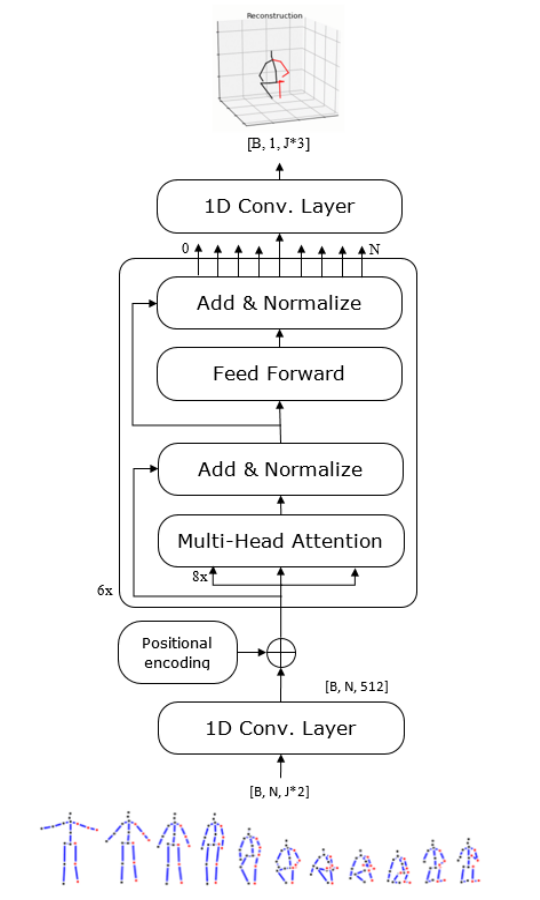
\includegraphics[height=2.2in]{images/model_3D.png}}
    \caption{Modelo Estimación de Pose 3D. Al igual de ViT usa solo capas con Decoders. Las entradas
             son las estimaciones 2D de algún otro predictor o los GT.}
    \label{fig:m3d}
\end{figure}

\end{frame}
%---------------------------------------------------------

%---------------------------------------------------------
\begin{frame}
\frametitle{Modelo Estimación de Pose 3D}

\begin{figure}[htbp]
    \centerline{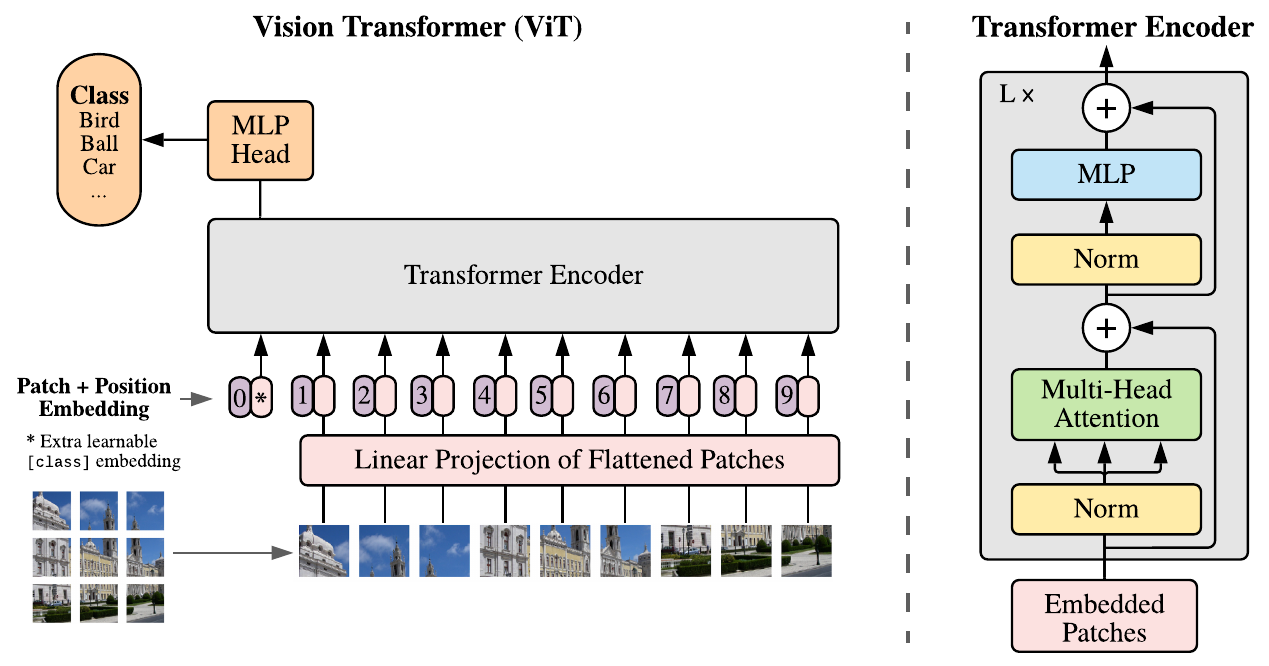
\includegraphics[height=2.0in]{images/model_vit.png}}
    \caption{Modelo ViT usado en las tareas de clasificación de enfermedades
             pulmonares. La entrada es una secuencia obtenida al dividir la imagen
             en pequeños parches.}
    \label{fig:vit}
\end{figure}

\end{frame}
%---------------------------------------------------------

\section{Variación a Transformes: Cabezas de Atención Flexibles}

\begin{frame}
\frametitle{MultiHead-Self-Attention}
El Transformer está basado en la idea de Multihead-Self-Attention (MHA), permitiendo al modelo
conjuntamente atender a información en diferentes posiciones desde diferentes subespacios de
representación.

\begin{equation*}
    mha(Q, K, V) = Concat(head_1,head_2,head_3,..., head_h)W^O
\end{equation*}

donde $Q, K, V \in \mathbb{R}^{nxd_{m}}$ son embeddings de entrada, $n$ es el tamaño de la
secuencia, $d_m$ es el tamaño del embedding y $h$ el número de cabezas de atención. Cada cabeza es
definida como sigue:

\begin{equation*}
    head_i = Attention(QW_i^Q, KW_i^K, VW_i^V) = sofmax\Big(\frac{QW_i^Q (KW_i^K)^T}{\sqrt{d_k}}\Big) VW_i^V
\end{equation*}

donde $W_i^Q$, $W_i^K$ $\in \mathbb{R}^{d_mxd_k}$, $W_i^V$ $\in \mathbb{R}^{d_mxd_v}$, $W^O$
$\in \mathbb{R}^{hd_vxd_m}$ y $d_k=d_v=d_m/h$

\end{frame}

\begin{frame}
\frametitle{MultiHead-Self-Attention}

\begin{itemize}
    \item El tamaño de la cabeza es dependiente de la dimensión del embedding y el número de cabezas
          de atención.
    \item Mientras más cabezas de atención los embeddings son proyectados a dimensiones cada vez
          más bajas, lo que implica un compresión y perdida de información.
    \item Escalar el modelo un poco más costoso en memoría y costo computacional.
    \item Redefiniendo
\end{itemize}

\end{frame}

\end{document}
